\section{Results}

Table~\ref{tab:sota} reports hit-rate at matched false-serve budgets for the fixed similarity threshold, the vCache reimplementation, and SERVE on the 100k MiniLM QQP corpus with a 60k-entry cache, averaged over 4 seeds.
% E2
SERVE matches or exceeds both baselines at every budget swept.
% E2
At the strictest budget, $\beta \le 0.5\%$, SERVE reaches 0.0238, a +17.9\% relative gain over the fixed threshold (0.0202) and +9.9\% over vCache (0.0216).
% E2
At the primary $\beta \le 1\%$ operating point, hit-rate rises from 0.0338 (fixed, std~0.0019) to 0.0355 (vCache, std~0.0005) to 0.0378 (SERVE, std~0.0017), corresponding to relative gains of +11.9\% and +6.5\%.
% E2
The separation narrows as the budget loosens: at $\beta \le 2\%$, SERVE achieves 0.0590 (+6.6\% over fixed, +4.6\% over vCache), and at $\beta \le 5\%$ the methods converge at 0.0993 for both SERVE and vCache (0.0983 for fixed, a +1.0\% and +0.1\% edge).
% E2
The monotonic widening of the gap as budgets tighten is the headline pattern: the stricter the reliability constraint, the more headroom margin awareness creates over a scalar similarity cutoff.

All reported results use the 20k gate-training split for threshold and budget calibration; the selected operating points are applied to the held-out 20k test split without adjustment, preserving an out-of-sample evaluation for every method.
% E12
Each hit-rate is a proportion on $n = 20{,}000$ test queries; the 95\% binomial confidence interval (Wald) for a mean hit-rate $\hat{p}$ is approximately $\hat{p} \pm 1.96 \sqrt{\hat{p}(1{-}\hat{p}) / n}$.
% E12
At $\beta \le 0.5\%$, the intervals are: SERVE 0.0238 [0.0217, 0.0259], vCache 0.0216 [0.0196, 0.0236], Fixed 0.0202 [0.0183, 0.0222].
% E2
At $\beta \le 1\%$: SERVE 0.0378 [0.0352, 0.0405], vCache 0.0355 [0.0329, 0.0381], Fixed 0.0338 [0.0313, 0.0363] (seed-to-seed std reported in Table~\ref{tab:sota}).
% E2
At $\beta \le 2\%$: SERVE 0.0590 [0.0557, 0.0623], vCache 0.0564 [0.0532, 0.0596], Fixed 0.0553 [0.0521, 0.0585].
% E2
At $\beta \le 5\%$: SERVE and vCache 0.0993 [0.0952, 0.1035], Fixed 0.0983 [0.0942, 0.1024].
% E2
The SERVE-to-Fixed difference at $\beta \le 1\%$ is $+0.0040$ points, larger than the half-width of either CI, consistent with a systematic rather than sampling-driven gap.
% E2

\begin{table}[!t]
\centering
\caption{SERVE achieves higher hit-rate at every matched false-serve budget, with the largest relative gains concentrated at the strictest budgets.}
\label{tab:sota}
\begin{tabular}{lccccc}
\toprule
$\beta$ & Fixed & vCache & SERVE & vs.\ Fixed & vs.\ vCache \\
\midrule
$\le 0.5\%$ & 0.0202 & 0.0216 & \textbf{0.0238} & +17.9\% & +9.9\% \\
$\le 1\%$   & \begin{tabular}[t]{@{}c@{}}0.0338\\(0.0019)\end{tabular}
            & \begin{tabular}[t]{@{}c@{}}0.0355\\(0.0005)\end{tabular}
            & \begin{tabular}[t]{@{}c@{}}\textbf{0.0378}\\(0.0017)\end{tabular}
            & +11.9\% & +6.5\% \\
$\le 2\%$   & 0.0553 & 0.0564 & \textbf{0.0590} & +6.6\% & +4.6\% \\
$\le 5\%$   & 0.0983 & 0.0993 & \textbf{0.0993} & +1.0\% & +0.1\% \\
\bottomrule
\end{tabular}
\end{table}

Aggregate ROC-AUC is nearly identical across the three methods: 0.8948 for the fixed threshold, 0.8963 for vCache, and 0.8967 for SERVE.
% E3
The fixed threshold already separates the bulk of the similarity distribution well. The entire contest sits in the low-false-serve tail, the region where a production cache with a low tolerance for wrong answers is constrained to operate. A summary statistic that averages over all operating points hides the regime where the decision rule actually matters: the gain comes from a cleaner decision boundary at low false-serve rates, not from improved overall separation.

\begin{figure}[!t]
\centering
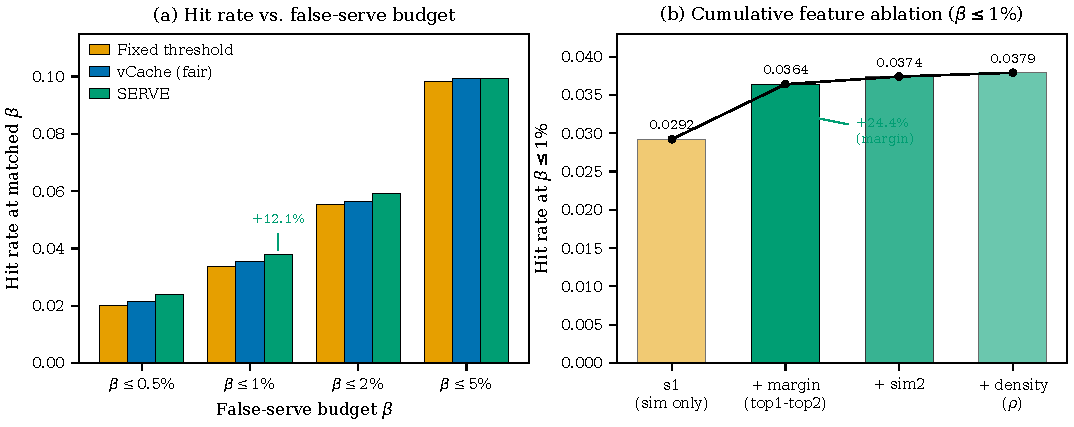
\includegraphics[width=\columnwidth]{figures/fig1_sota_ablation.pdf}
\caption{SERVE achieves higher hit-rate at matched false-serve budgets compared to fixed-threshold and vCache baselines; ablation reveals that the margin feature alone recovers 83\% of the total improvement.}
\label{fig:fig1_sota_ablation}
\end{figure}

Table~\ref{tab:ablation} decomposes the gain by adding features to the gate one at a time.
% E4
A similarity-only gate reaches 0.0292 at $\beta \le 1\%$, somewhat below the 0.0338 fixed-threshold baseline; the tree ensemble's piecewise-constant scores quantize the operating frontier at strict budgets, costing a few points relative to a continuous threshold.
Adding the margin $m$ raises hit-rate to 0.0363, a +24.4\% relative jump.
% E4
Adding the runner-up similarity $s_2$ contributes a further +2.9\% (to 0.0374), and local density $\rho$ a final +1.1\% (to 0.0378).
% E4
The margin alone recovers 83\% of SERVE's total improvement over a similarity-only gate.
% E4
One specific, already-computed quantity, the gap between the best match and the runner-up, does nearly all of the work that similarity alone cannot do.

\begin{table}[!t]
\centering
\caption{Feature ablation at $\beta \le 1\%$. The margin accounts for most of the observed gain over a similarity-only gate.}
\label{tab:ablation}
\begin{tabular}{lccc}
\toprule
Features & Hit-rate & $\Delta$ from $s_1$ & Share \\
\midrule
$s_1$ only & 0.0292 & -- & -- \\
$s_1, m$ & 0.0363 & +0.0071 & 83\% \\
$s_1, m, s_2$ & 0.0374 & +0.0082 & 95\% \\
$s_1, m, s_2, \rho$ & \textbf{0.0378} & +0.0086 & 100\% \\
\bottomrule
\end{tabular}
\end{table}

The gate adds 0.8\,$\mu$s per query in batched inference (std~0.0 across 4 runs, Apple M-series CPU), confirming that the computational cost is negligible relative to embedding computation, nearest-neighbor search, and LLM inference.
% E5

\begin{figure*}[!t]
\centering
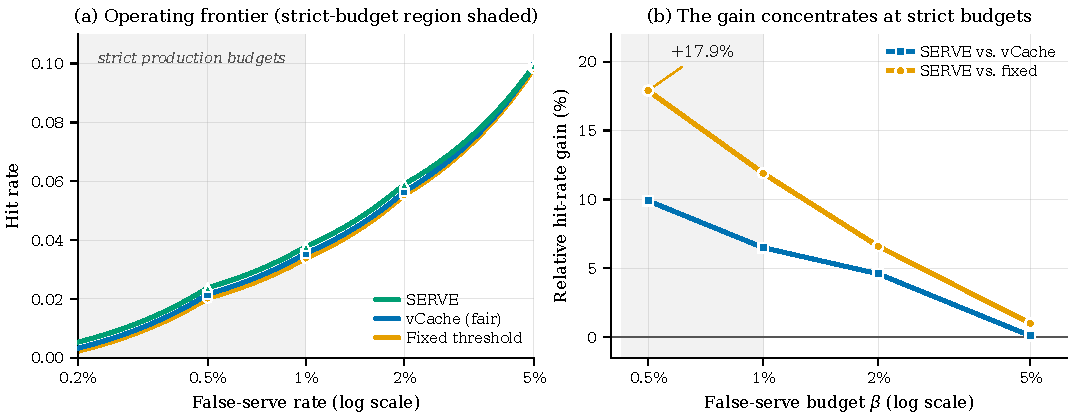
\includegraphics[width=\textwidth]{figures/fig2_frontier.pdf}
\caption{SERVE dominates the hit-rate versus false-serve frontier at low budgets, with the separation between methods widening monotonically as the budget tightens.}
\label{fig:fig2_frontier}
\end{figure*}

The margin proves dominant, but the aggregate results leave open the question of when and how it separates correct serves from incorrect ones. These results are demonstrated on paraphrase and adversarial paraphrase corpora (QQP, PAWS) with sentence-transformers (MiniLM, mpnet). The next section characterizes the operating regimes where the advantage is largest and examines the decision boundary the gate learns.
